\chapter{Motion and Work in Living Systems}
\thispagestyle{fancy}
\fancyhead[RE,LO]{Experiment \thechapter}
%
%\section{Classifying Motion and Examining Work in Onion Cells.}
%\section*{Introduction}
Plant cells store information, food, and waste in small bubbles called vesicles.
These vesicles are transported throughout cells using a combination of mechanisms.
They move throughout cells utilizing random motion, as we have studied previously.
Diffusion is far too slow a mechanism to transport important materials over long distances though, so cells have developed a series of complex mechanisms for directed motion.
In many cells, motor proteins transport vesicles along pathways framed by cytoskeletal fiber.
One such process involves vesicles being transported by myosin motors along actin filaments.
Another involves kinesin motors carrying vesicles along microtubules.
Directed motion is also observed in a process called cytoplasmic streaming, where the vesicles and other material inside a cell moves due to a fluid flow.

\begin{wrapfigure}{r}{0.5\textwidth}
  \vspace{-20pt}  
  \begin{center}
    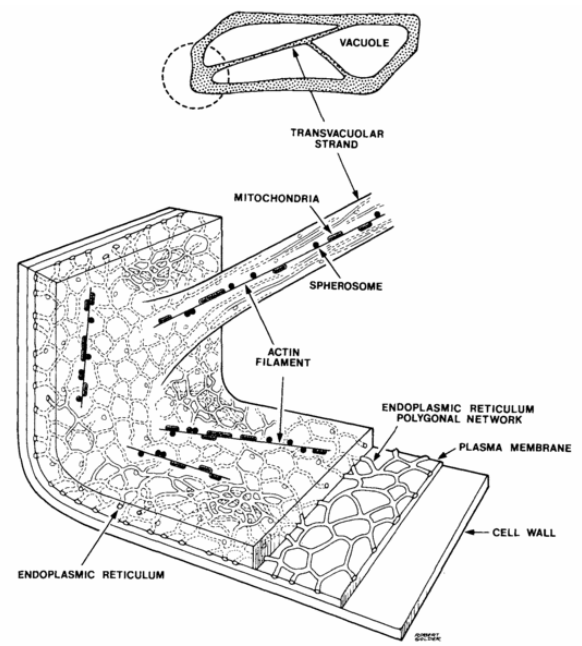
\includegraphics[width=0.48\textwidth]{cellWall}
  \end{center}
  \caption{Inside a cell wall.}
  \label{fig:cell-wall}
  \vspace{-20pt}
\end{wrapfigure}

All of these types of motion can be observed in onion cells.
Therefore, onion cells are a cheap and simple experimental subject that allows us to make several interesting observations.
By looking at individual onion cells, we can make both qualitative and quantitative observations about the different types of motion.
Moreover, analysis of the work required to move the vesicle [based on terminal speed and energy required for ATP hydrolysis (23 kJ/mole), with the step size and efficiency of the motor] can give us insight into the effective viscosity and probable structure of the cytosol (intracellular medium).

\paragraph{For this two week lab:} The goal of this experiment is to understand how quantitative analysis of biological phenomena can provide insight into the structure of living systems. You should aim to capture enough video so that you can fully characterize the motion of around 10 different vesicles. You will use these tracks to model work and power in a physical, living system.
\begin{enumerate}
\item Make sure that you understand how to safely operate the microscope, how to capture video with the microscope, and the pixel-to-distance ratio of the microscope camera.
\item Capture your first videos and do a preliminary analysis.
\item Discuss as a class the method you plan to use to analyze your videos.
\item Collect additional videos if necessary.
\item Analyze your video(s) to characterize the motion of the vesicles.
\end{enumerate}

\subsection*{Investigation}
In order to observe motion inside of individual onion cells, we must first prepare a slide with one layer of onion cells:
\begin{enumerate}
\item Cut down to the center of the onion (activity in the onion cells is dependent on distance from the surface of the onion, thus the center is typically more active). 
\item Once you have a layer of onion close to the center, peel the lower cell membrane off of it( the cell membrane is relatively strong, and is made up of a single layer of cells). 
\item Put a few drops of saline solution down on a slide, place your onion membrane down, and then put a few more drops of saline solution down. 
\item Cover it with a slide cover, and blot the remaining saline solution. 
\item Keep in mind that onions are actually alive, but when you cut into it and mount the membrane on a slide, the cells will slowly die. The lifespan of cells in these slides is around 30 minutes. You might not observe cell activity on the first try; sometimes it will be necessary to try another section of the onion, or even another onion. 
\item Once you have successfully prepared an onion slide, look around to observe all the activity in the cells. You can explore different layers within the cells by changing the focus of the microscope. Most of the interesting activity will be happening at the top or bottom layer of cells. 
\item Find regions where vesicles appear to be moving randomly, and compare them to regions where vesicles appear to be directed somehow. 
\item Take a video or two (be sure to note and record the frame rate for the video) that show both apparently random and apparently directed motion. 
\item Track particles using particle tracking in ImageJ and analyze the two groups of motion using the techniques we have developed so far in the lab. 
\item Before you leave ImageJ, also measure the SIZE of the vesicles (you will need this if you begin working toward the diffusion constant or resistive forces).
\end{enumerate}

\subsection*{Interpretation}
After you have observed the motion both quantitatively and qualitatively, you should be able to make some interesting statements about the motion of vesicles in cells.
\begin{itemize}
\item Is the apparently random motion of vesicles really random or is it confined? Or does vesicle motion look random because vesicles fall off of their ``tracks'' frequently?
\item Where do random motion and active transport occur in cells?
\item How do the velocities of vesicles moving randomly and actively differ?
\item What is the advantage cells gain in utilizing both random motion and active transport of vesicles? When is active transport advantageous, when random motion?
\end{itemize}
Once you have measured the \textbf{average radius} and \textbf{average speed} for the group of vesicles experiencing directed motion, you can do an analysis of energetic concerns to calculate the \textbf{rate of ATP hydrolization} (R) and the \textbf{effective viscosity} ($\mu$) of the cytosol. From the effective viscosity of the cytosol, what can you conclude about the nature and structure of the cytosol? Here are some numbers and equations that might help:
\begin{itemize}
\item Average size of a myosin motor 'step' = 10 nm, stepping along an actin filament.
\item Average size of a kinesin motor 'step' = 8 nm, stepping across/along a tubulin dimer.
\item One 'step' for a motor is equivalent to 1 ATP hydrolization cycle (23 kJ/mole).
\item For both myosin motors and kinesin, the efficiency (work produced $\div$ energy consumed) is 60\%.
\end{itemize}
As you will learn in class shortly, since the vesicle does not change speed, the work being put in (produced by the motor) is being consumed (dissipated) by the viscous resistance within the cytosol.
%With this knowledge, and the following helpful equations, you should be able to determine the effective viscosity of the cytosol and the rate of ATP hydrolysis.
The `efficiency' of a vesicle's motion can be calculated with
\begin{equation}
e = \frac{W_{produced}}{E_{consumed}} = \frac{P_{produced}}{P_{consumed}}
\end{equation}
where W is the work done by the vesicle (in moving itself), E is the energy of one ATP cycle.
This is directly equivalent to the ratio between the power produced and consumed by these entities.
The power consumed by a vesicle can be calculated with
\begin{equation}
P_{consumed} = \frac{N \cdot E}{t} = R \cdot E
\end{equation}
where N is number of ATP cycles, E is the energy of one ATP cycle, t is the time interval. R is the rate of hydrilization.
\begin{equation}
P_{produced} = \frac{F \cdot d}{t} = F \cdot v
\end{equation}
where F is the force generated by the vesicle and d is the displacement.
Displacement divided by time is just the velocity, $v$, of the particles, and can be related to the rate of hydrilization like so:
\begin{equation}
v = \frac{d}{t} = \frac{N \cdot s}{t} = R \cdot s
\end{equation}
where s is the step size.
\par
You also need to consider the viscous force acting on the particles. This can be calculated with \emph{Stoke's Law}, which takes the following form:
\begin{equation}
F_{viscous} = -6 \pi \mu r v
\end{equation}
where $\mu$ is the viscosity, r is the vesicle radius, and v is the speed of the vesicle.
%For comparison, the viscosity of DI water is $8.6 \times 10^{-4}$ Pa$\cdot$s at room temperature (27 $^{\circ}$C).

%For P = Power, W = Work, t = time interval, E = Energy of one ATP cycle, \# = number of ATP cycles, R = rate of ATP hydrolization, e = efficiency, F = force, d = displacement, v = speed of vesicle, s = step size, $\mu$ = viscosity, and r = vesicle radius, the following are true: